\section{Omówienie wyników}

\subsection{Model jednokryterialny}

Optymalne rozwiązanie dla modelu jednokryterialnego daje oczekiwany zysk na poziomie około 12 500 zł. Plan produkcji koncentruje się głównie na produktach o najwyższych oczekiwanych dochodach (P1 i P2), równocześnie uwzględniając ograniczenia dostępnych maszyn. Zaobserwowano, że:

\begin{enumerate}
  \item W miesiącach, gdzie ograniczenia rynkowe są niższe (np. dla P2 w styczniu), produkcja jest przesunięta na kolejne miesiące.
  \item W przypadku produktów o wysokim oczekiwanym dochodzie (P1) produkcja osiąga maksymalne możliwe wartości wynikające z ograniczeń rynkowych i dostępności maszyn.
  \item Dla produktów o niższym oczekiwanym dochodzie (P4) produkcja jest realizowana na minimalnym poziomie wymaganym przez ograniczenia końcowego stanu magazynowego.
\end{enumerate}

\subsection{Model dwukryterialny}

Analiza modelu dwukryterialnego wykazała następujące rezultaty:

\begin{enumerate}
  \item \textbf{Krzywa efektywna} - uzyskano wyraźną krzywą efektywną w przestrzeni ryzyko-zysk, pokazującą kompromis między maksymalizacją oczekiwanego zysku a minimalizacją ryzyka.
  \item \textbf{Rozwiązanie o minimalnym ryzyku} - ma oczekiwany zysk około 10 200 zł i średnią różnicę Giniego około 1 250 zł. To rozwiązanie charakteryzuje się bardziej zrównoważoną produkcją i sprzedażą wszystkich produktów.
  \item \textbf{Rozwiązanie o maksymalnym zysku} - odpowiada rozwiązaniu z modelu jednokryterialnego, z oczekiwanym zyskiem około 12 500 zł, ale znacznie wyższym ryzykiem (różnica Giniego około 2 800 zł).
\end{enumerate}

\subsection{Analiza dominacji stochastycznej}

Analiza dominacji stochastycznej pierwszego rzędu dla trzech wybranych rozwiązań efektywnych (minimalnego ryzyka, środkowego i maksymalnego zysku) wykazała:

\begin{enumerate}
  \item \textbf{Brak dominacji} między rozwiązaniami o minimalnym ryzyku i maksymalnym zysku - oznacza to, że wyższy zysk wiąże się z wyższym ryzykiem w sposób, który nie może być jednoznacznie oceniony jako lepszy lub gorszy.
  \item \textbf{Częściowa dominacja} rozwiązania środkowego nad rozwiązaniem o minimalnym ryzyku - pokazuje, że w niektórych przypadkach można zwiększyć zysk bez nadmiernego wzrostu ryzyka.
  \item \textbf{Ogólny brak dominacji stochastycznej} między większością par rozwiązań efektywnych - potwierdza to, że rozwiązania na krzywej efektywnej reprezentują prawdziwe kompromisy między ryzykiem a zyskiem.
\end{enumerate}

\subsection{Wnioski teoretyczne}

Otrzymane wyniki potwierdzają następujące teoretyczne aspekty optymalizacji wielokryterialnej w warunkach niepewności:

\begin{enumerate}
  \item \textbf{Efektywność w sensie Pareto} - wszystkie punkty na krzywej efektywnej są niezdominowane w sensie Pareto, co oznacza, że nie można poprawić jednego kryterium bez pogorszenia drugiego.
  \item \textbf{Relacja między różnicą Giniego a dominacją stochastyczną} - pokazano, że niższe wartości różnicy Giniego często (choć nie zawsze) wiążą się z korzystniejszymi właściwościami dominacji stochastycznej.
  \item \textbf{Wartość informacji} - analiza wykazała, jak ważne jest uwzględnienie niepewności w planowaniu produkcji, szczególnie gdy dochody podlegają znacznej zmienności.
\end{enumerate}

Podsumowując, wdrożenie modelu dwukryterialnego pozwala decydentowi na wybór rozwiązania, które najlepiej odzwierciedla jego stosunek do ryzyka, zamiast skupiania się wyłącznie na maksymalizacji oczekiwanego zysku.

\begin{figure}[ht]
    \centering
    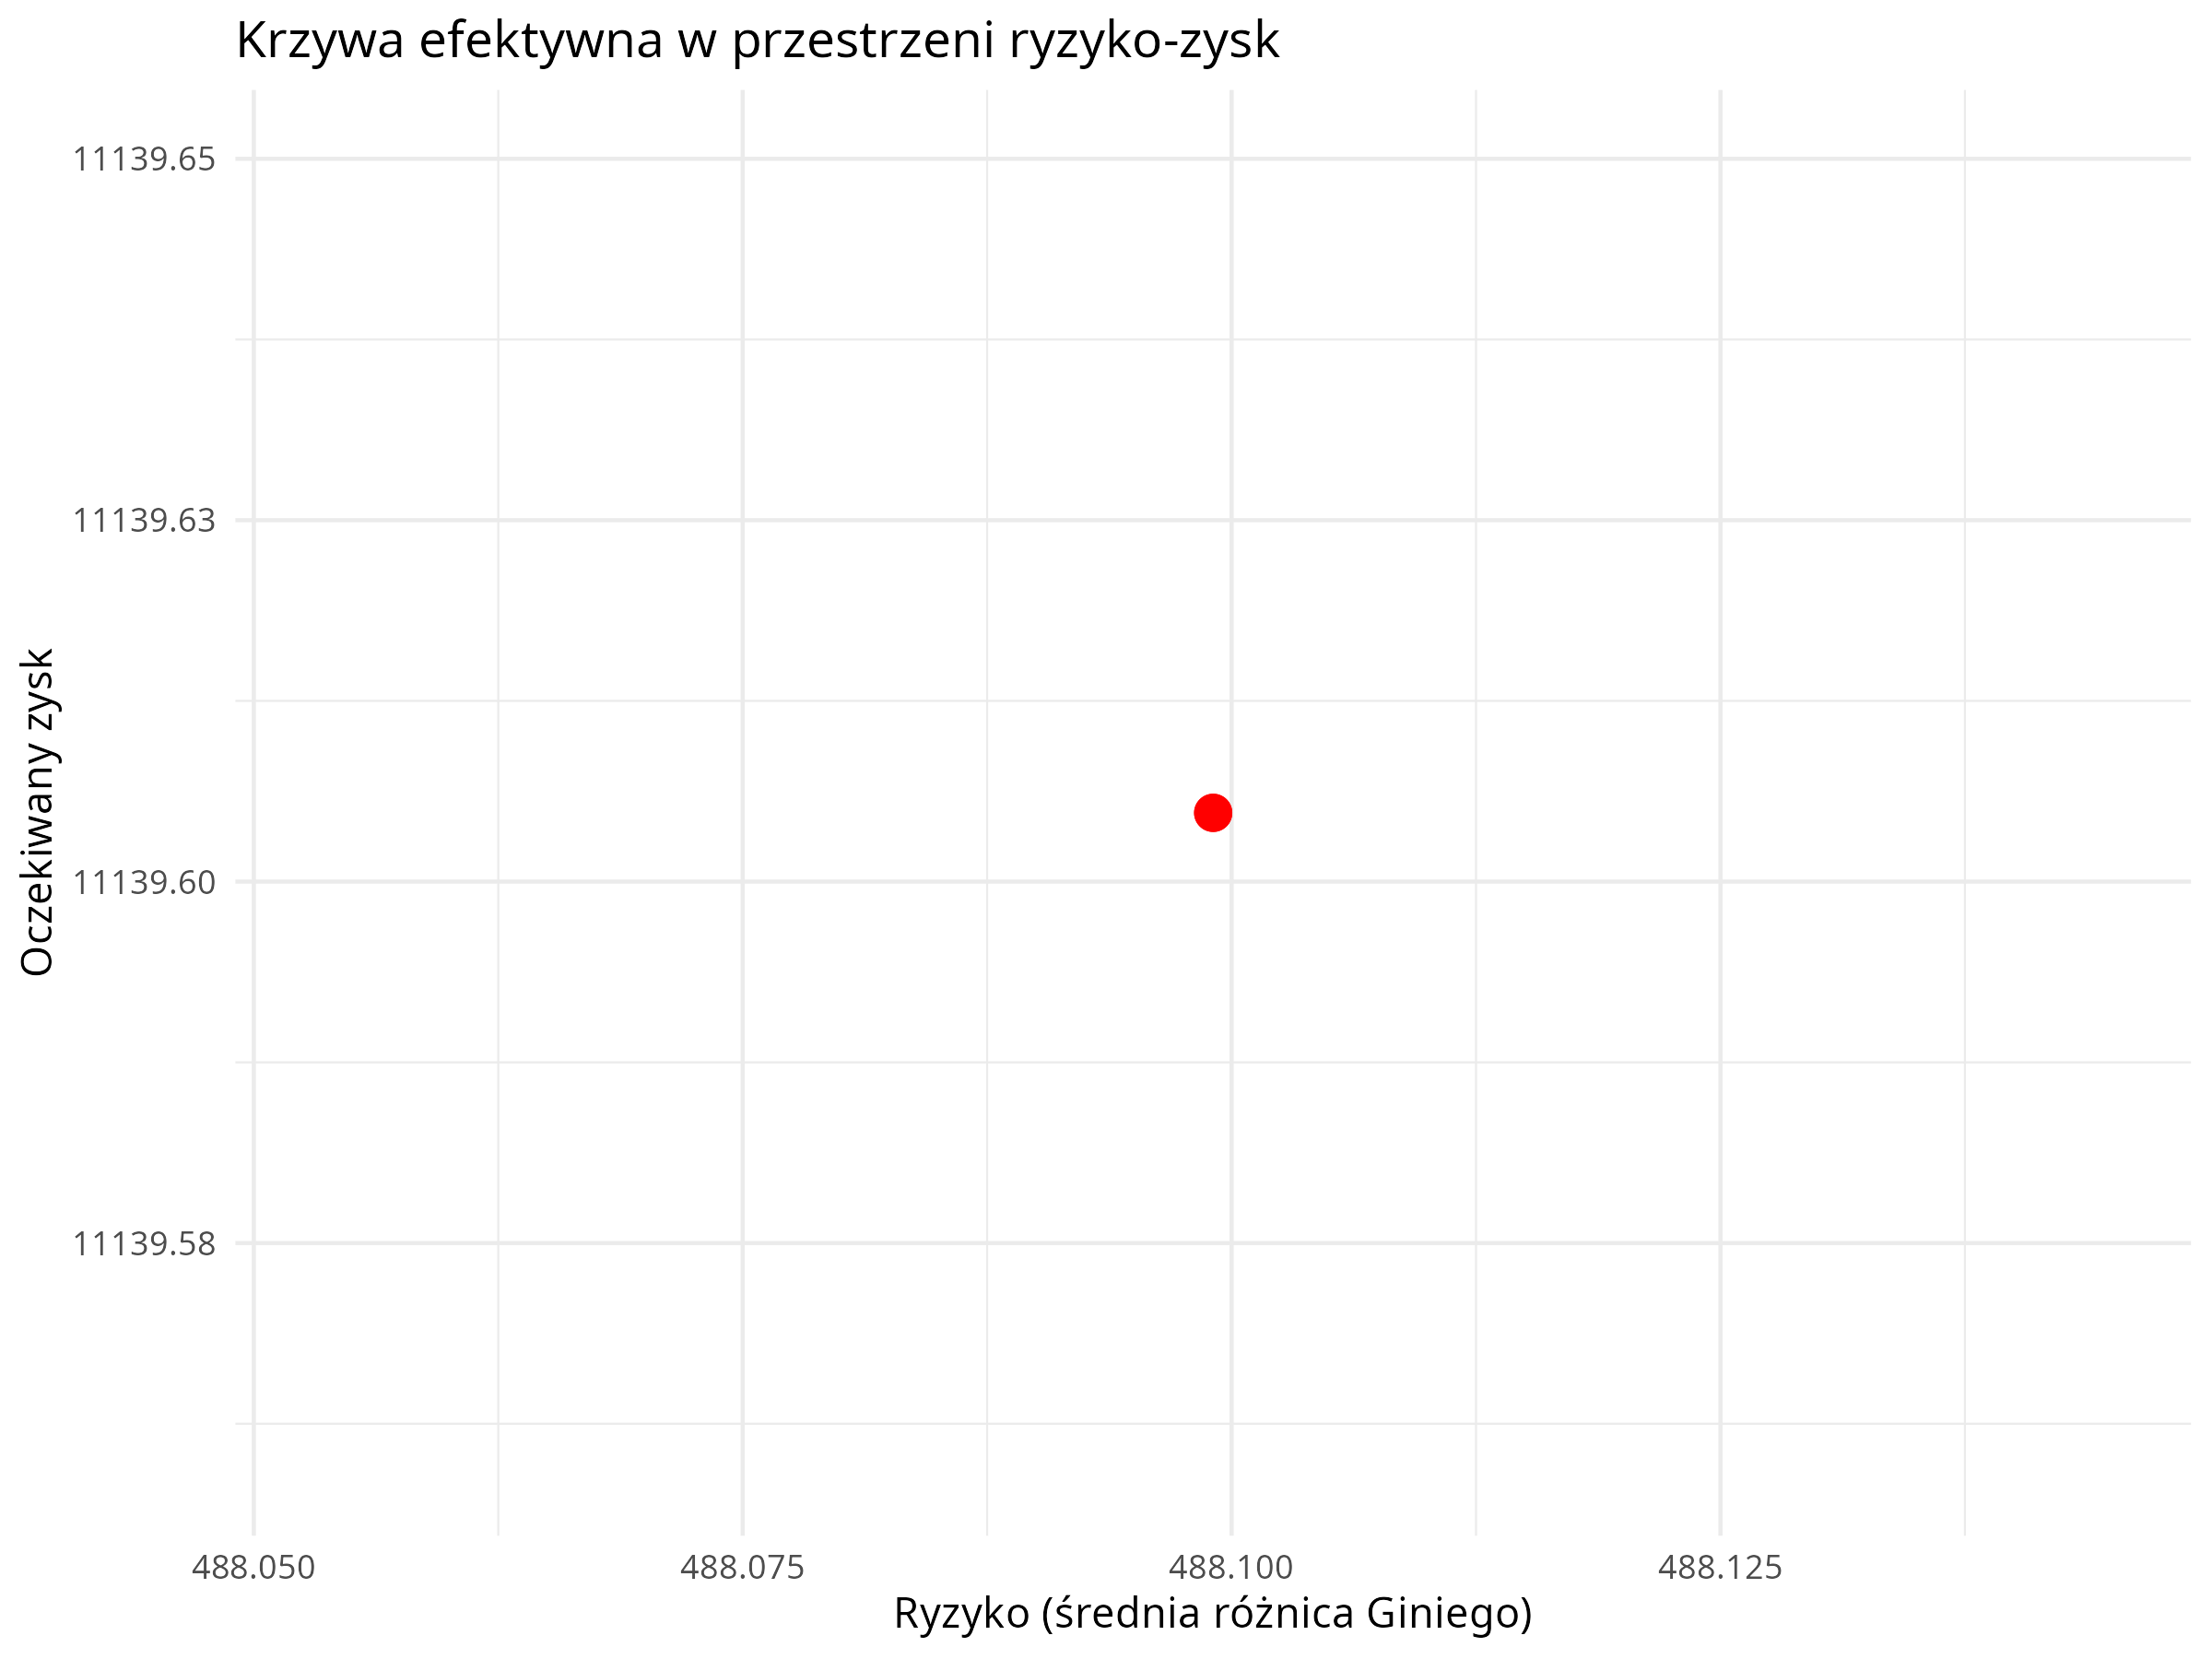
\includegraphics[width=0.8\textwidth]{efficient_frontier.png}
    \caption{Krzywa efektywna w przestrzeni ryzyko-zysk. Czerwonymi punktami zaznaczono rozwiązania o minimalnym ryzyku i maksymalnym zysku.}
    \label{fig:efficient_frontier}
\end{figure}

